\documentclass{beamer}
%
% Choose how your presentation looks.
%
% For more themes, color themes and font themes, see:
% http://deic.uab.es/~iblanes/beamer_gallery/index_by_theme.html
%
\mode<presentation>
{
  \usetheme{default}      % or try Darmstadt, Madrid, Warsaw, ...
  \usecolortheme{default} % or try albatross, beaver, crane, ...
  \usefonttheme{default}  % or try serif, structurebold, ...
  \setbeamertemplate{navigation symbols}{}
  \setbeamertemplate{caption}[numbered]
} 

\usepackage[english]{babel}
\usepackage[utf8]{inputenc}
\usepackage[T1]{fontenc}

\title[Your Short Title]{A Note on Risk-Limiting Bayesian Polling Audits for Two-Candidate Elections}
\author{Filip Zagórski}
\institute{Wroclaw University of Science and Technology}
\date{Date of Presentation}

\begin{document}

\begin{frame}
  \titlepage
\end{frame}

% Uncomment these lines for an automatically generated outline.
%\begin{frame}{Outline}
%  \tableofcontents
%\end{frame}

\section{Introduction}

\begin{frame}{Election Results Audits}

\begin{itemize}
  \item Election results audits sample ballots from a trustworthy paper trail to ensure that the reported winner really won.
\end{itemize}
\vskip .5cm
\begin{figure}
    \centering
    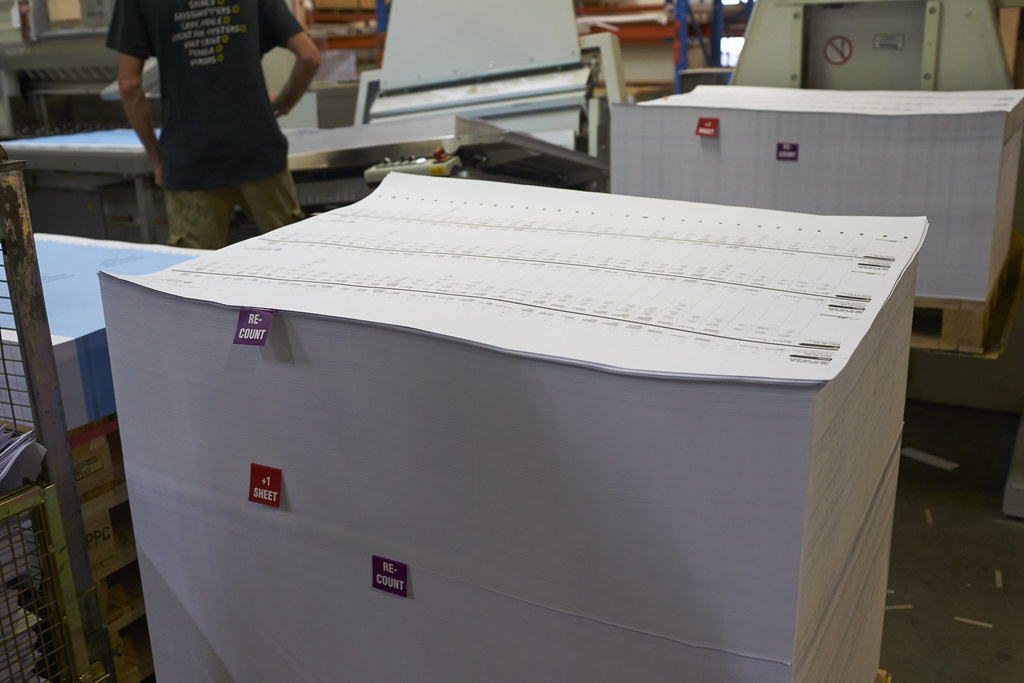
\includegraphics[width=200pt]{Paper_Ballot.jpg}
    \caption{Voter-verified paper ballots are the gold standard for election security and integrity. (Image Attribution: "Ballot Paper printing" by AusElectoralCom is licensed under CC BY-ND 2.0)}
    \label{fig:my_label}
\end{figure}
\end{frame}

\section{Some \LaTeX{} Examples}

\subsection{Tables and Figures}

\begin{frame}{Risk-Limiting Audits}
\begin{itemize}
    \item Risk-limiting audits aim to provide convincing statistical evidence that the reported winner really won. If they cannot, they proceed to a full hand count, revealing the true election outcome.
    \vskip 1cm
    \item If the reported outcome of the election is incorrect, the audit will fail to detect this (i.e., fail to proceed to a full hand count) at most only $\alpha \%$ of the time, where $\alpha$ is the risk limit.
    \vskip 1cm
    \item $\alpha$ bounds the worst-case risk.

\end{itemize}
\end{frame}

\begin{frame}{SPRT Risk-Limiting Audits}
\begin{itemize}
    \item The most popularly employed risk-limiting audit is the SPRT RLA, which is based on Abraham Wald's Sequential Probability Ratio Test.
    \vskip 1cm
    \item The SPRT RLA is a hypothesis test:
    \begin{itemize}
        \item $H_0 =$ The election was truly tied.
        \item $H_a =$ The election was won by the reported winner with $x$ fraction of the vote, $x > .5$.
    \end{itemize}
    \vskip 1cm
    \item Audit stops \& certifies winner $\iff$ $H_0$ rejected
\end{itemize}
\end{frame}

\begin{frame}{Likelihood Ratio of SPRT RLAs}
The likelihood ratio of the SPRT RLA is its test statistic. For SPRT RLAs with risk limit $\alpha$ and probability of proceeding to a full hand count unnecessarily $\beta$, the likelihood ratio is $$\sigma_n = \frac{p^{k_n} (1-p)^{n-k_n}}{(\frac{1}{2})^n}$$.
\begin{itemize}
    \item If $\sigma_n > \frac{1-\beta}{\alpha}$, stop the audit and certify the reported outcome.
    \item If $\sigma_n < \frac{\beta}{1-\alpha}$, proceed directly to a full hand count (to determine the true outcome).
    \item Otherwise, draw more samples.
\end{itemize}
    
\end{frame}

\begin{frame}{Bayesian Audits}
\begin{itemize}
    \item Bayesian audits also provide evidence that the reported winner really won.
    \vskip 1cm
    \item Bayesian audits assume a \emph{prior distribution} over all possible election tallies.
    \vskip 1cm
    \item The risk measure of a Bayesian audit, the "upset probability" or $\gamma$, is weighted by the prior.
\end{itemize}
\end{frame}
\begin{frame}{A Prior for A Bayesian Audit}
\begin{figure}
    \centering
    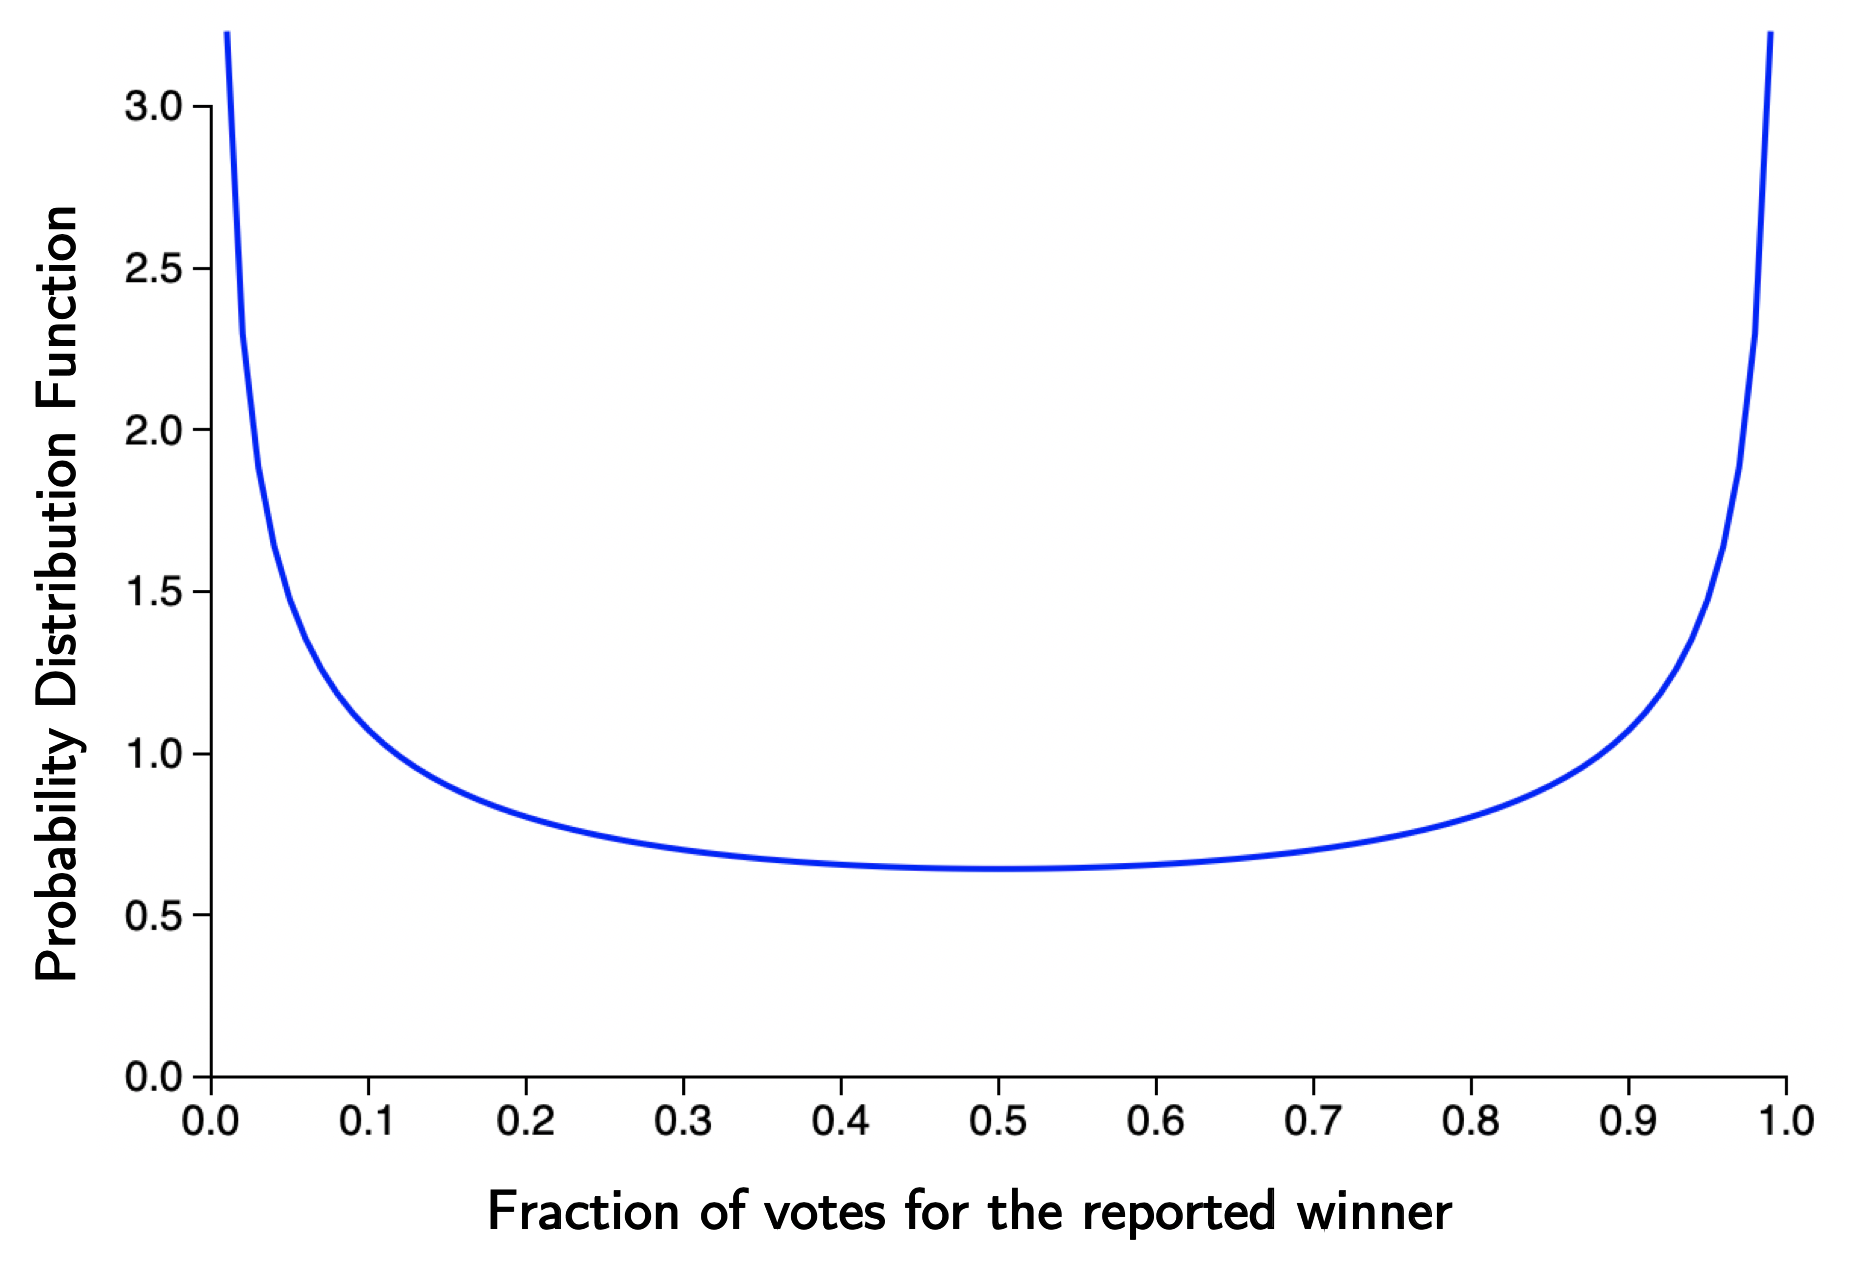
\includegraphics[width=200pt]{Beta_Prior.png}
    \caption{This prior assumes that landslide victories are more likely than tight races.}
    \label{fig:my_label}
\end{figure}
\end{frame}

\begin{frame}{Comparing Bayesian Audits and RLAs}
\begin{itemize}
    \item Similarities
    \begin{itemize}
        \item Stop certify reported winner only after considerable evidence for her winning.
        \item Require paper trails.
        \item Number of ballots polled is a random variable.
    \end{itemize}
    \vskip 1cm
    \item Differences
    \begin{itemize}
        \item RLAs bound the worst-case risk; Bayesian audits, an average-case risk.
        \item Bayesian audits are generally computed with simulation.
    \end{itemize}
\end{itemize}
\end{frame}

\begin{frame}{Our Contributions}
\begin{itemize}
    \item 1. Likelihood Ratio for Bayesian Audits
    \vskip 1cm
    \item 2. SPRT RLA as a Bayesian Audit
    \vskip 1cm
    \item 3. Bayesian Audits are Comparison Tests
    \vskip 1cm
    \item 4. The Bayesian RLA
\end{itemize}
\end{frame}

\begin{frame}{Likelihood Ratio for Bayesian Audits}
\emph{NOTE: The likelihood ratio for Bayesian audits is not present in the short paper; only a mention that Bayesian audits need not be performed with simulation.}

Recall the likelihood ratio for the for the SPRT RLA:
    $$\frac{p^{k_n} (1-p)^{n-k_n}}{(\frac{1}{2})^n}$$

We can exhibit the Bayesian RLA in a similar form:
    $$\frac{\sum_{x=\frac{N}{2}+1}^N p^{k_n} (1-p)^{n-k_n} f_X(x)}{\sum_{x=0}^{x=\frac{N}{2}} p^{k_n} (1-p)^{n-k_n} f_X(x)}$$

\begin{itemize}
    \item $N =$ total votes cast for the two candidates
    \item $n =$ sample size
    \item $k_n =$ votes for reported winner in sample of size $n$
    \item $p = x/N$
    \item $f_X$ is the prior.
\end{itemize}
\end{frame}

\begin{frame}{The SPRT RLA is a Bayesian Audit}
\begin{itemize}
    \item The $(\alpha, \beta, p)$-SPRT RLA is the SPRT RLA with risk limit $\alpha$, probability of proceeding directly to a hand count unnecessarily $\beta$, and reported winner vote share (less a small tolerance) $p$.
    \item The $(\gamma, f_X)$-Bayesian Audit is the Bayesian audit with upset probability bound $\gamma$ and prior $f_X$.
\end{itemize}
\vskip 1cm
Result: The $(\gamma, \gamma, p)$-SPRT RLA with/without replacement is the $(\gamma, f_X)$-Bayesian audit, where $f_X = \frac{1}{2} \delta_{x,\frac{N}{2}} + \frac{1}{2} \delta_{x,pN}$.
\end{frame}

\begin{frame}{The Implicit Prior of the SPRT RLA}
\begin{figure}
    \centering
    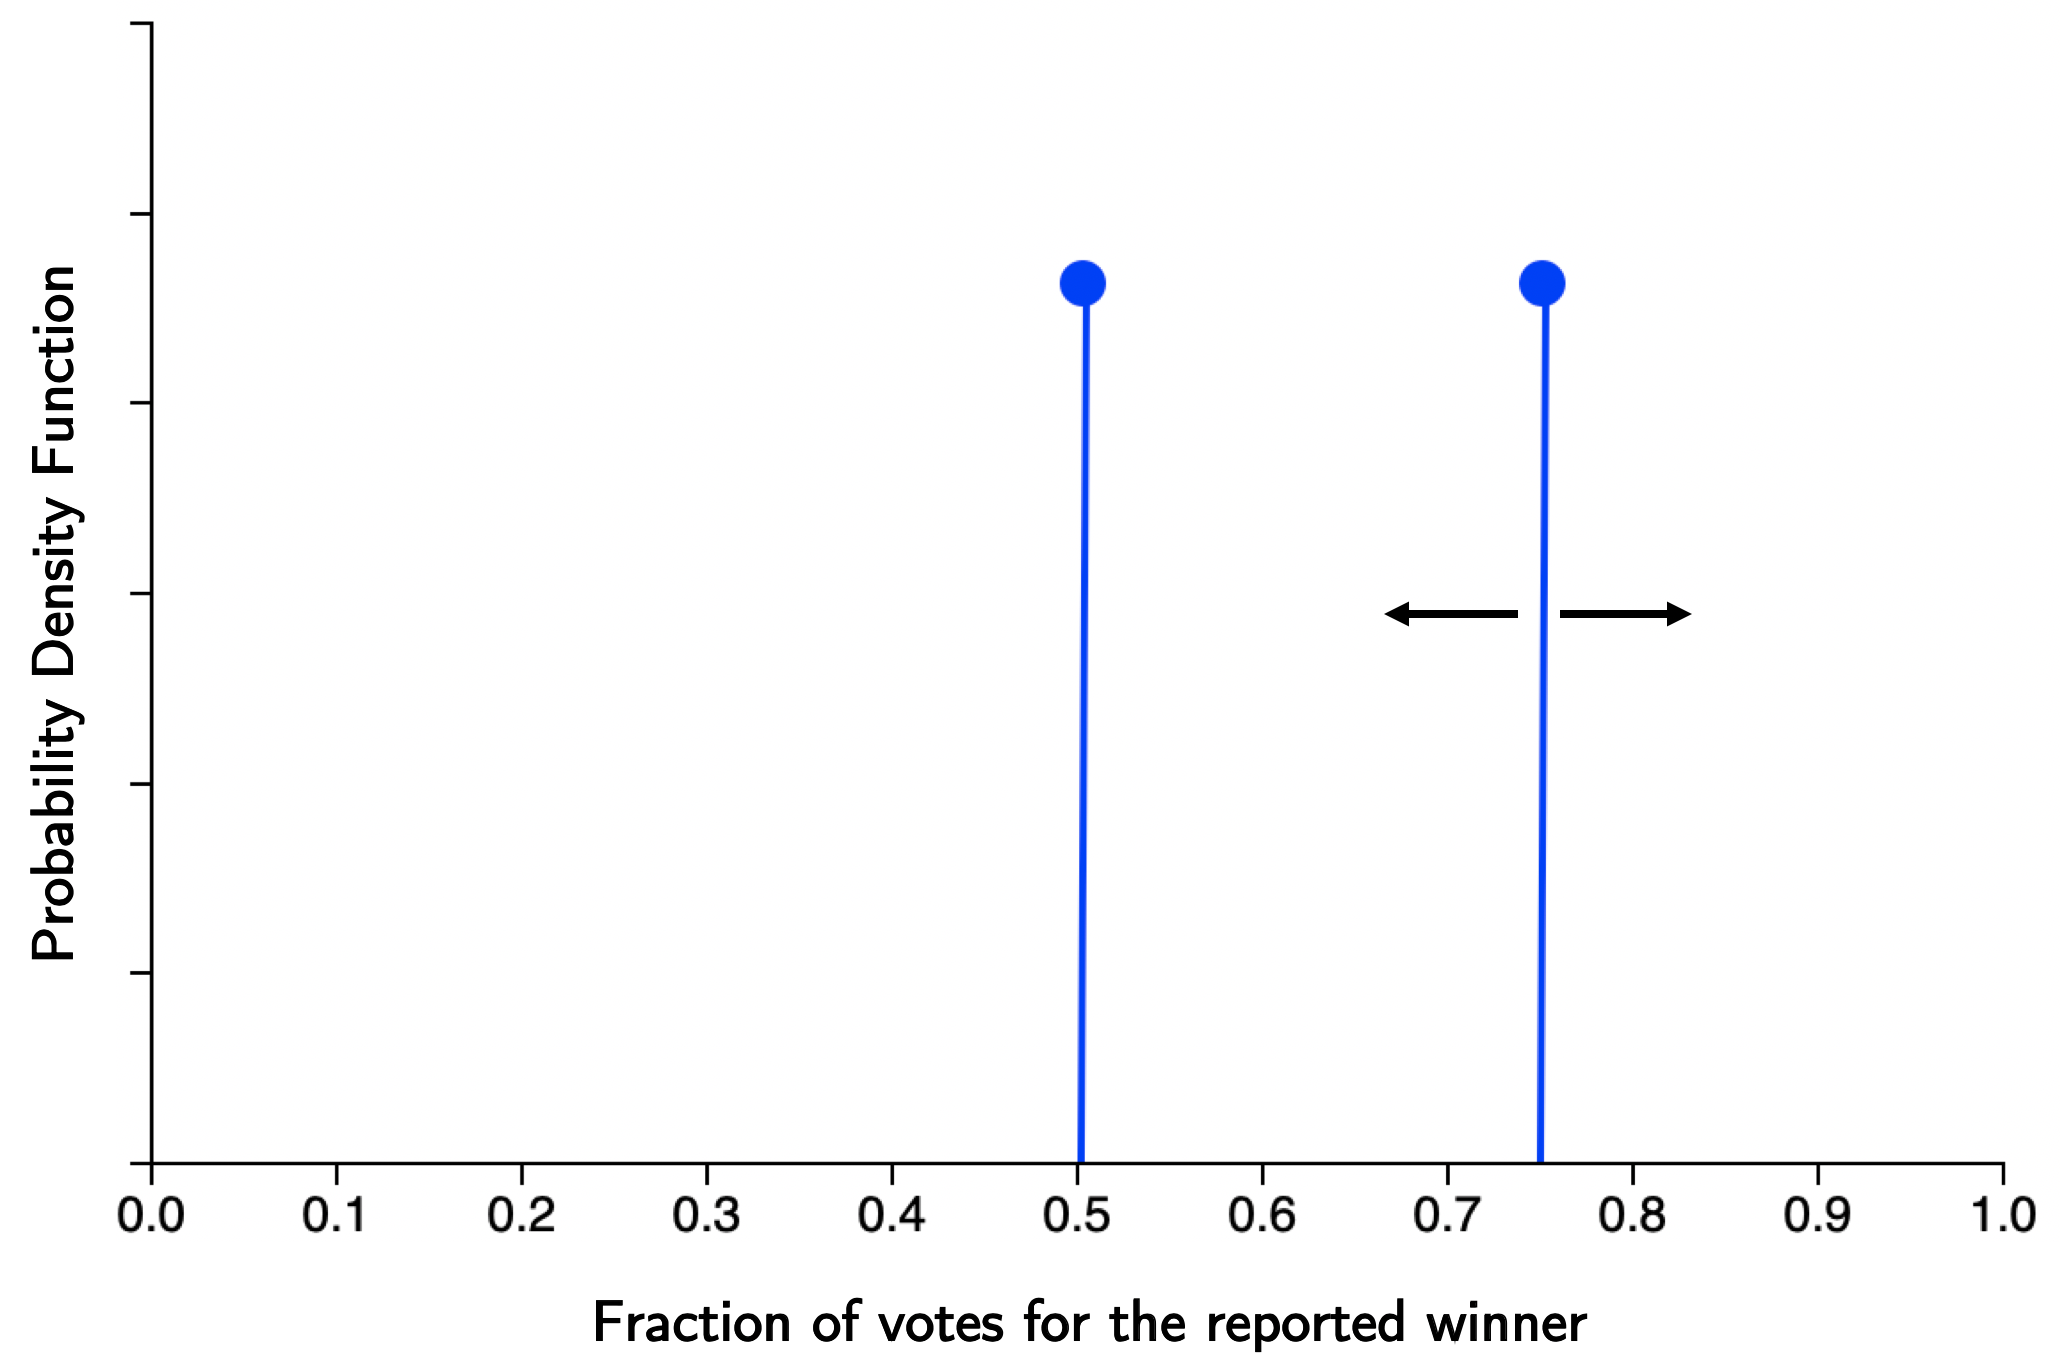
\includegraphics[width=200pt]{SPRT_Prior.png}
    \caption{The left $\delta$ function is fixed at $x = .5$, but the right $\delta$ function is not, and depends on the reported winner's reported vote share.}
    \label{fig:my_label}
\end{figure}
\end{frame}

\begin{frame}{The Bayesian Audit is a Comparison Test}
Result: For Bayesian audits computed without simulation, the decision rule is a comparison test (like the SPRT RLA!).
\vskip 1cm
We simply compare the number of ballots for the reported winner in the sample, $k_n$, to predetermined decision boundaries, $k_{min}(n)$ and $k_{max}(n)$, $k_{min}(n) > k_{max}(n)$.
\begin{itemize}
    \item If $k_n \geq k_{min}(n)$, stop the audit and certify the reported outcome.
    \item If $k_n \leq k_{max}(n)$, proceed directly to a full hand count.
    \item Otherwise, continue drawing samples.
\end{itemize}
\end{frame}

\begin{frame}{The Bayesian RLA}
Given a prior for a Bayesian audit $f_X$, define $f_X^*$ as follows:
\begin{equation}
f_X^* =  \left\{ \begin{array}{ll} f_X(x) & ~~~ x > \frac{N}{2}\\
& \\
\frac{1}{2}& ~~~ x=\frac{N}{2} \\
& \\
0 & ~~~else \\
\end{array}
\right .
\label{eqn:f_X*}
\end{equation}
\begin{theorem}
The $(\alpha, f_X^*)$-Bayesian Audit is an $\alpha$-{\em RLA} with $P_U < \alpha$ for election $E$ with prior $f_X$ and is a most efficient audit achieving $P_M < \alpha$ and $P_U < \alpha$ for the prior $f_X^*$.
\end{theorem} 
\end{frame}

\begin{frame}{Before and After: Making a Prior Risk-Limiting}
\begin{figure}
    \centering
    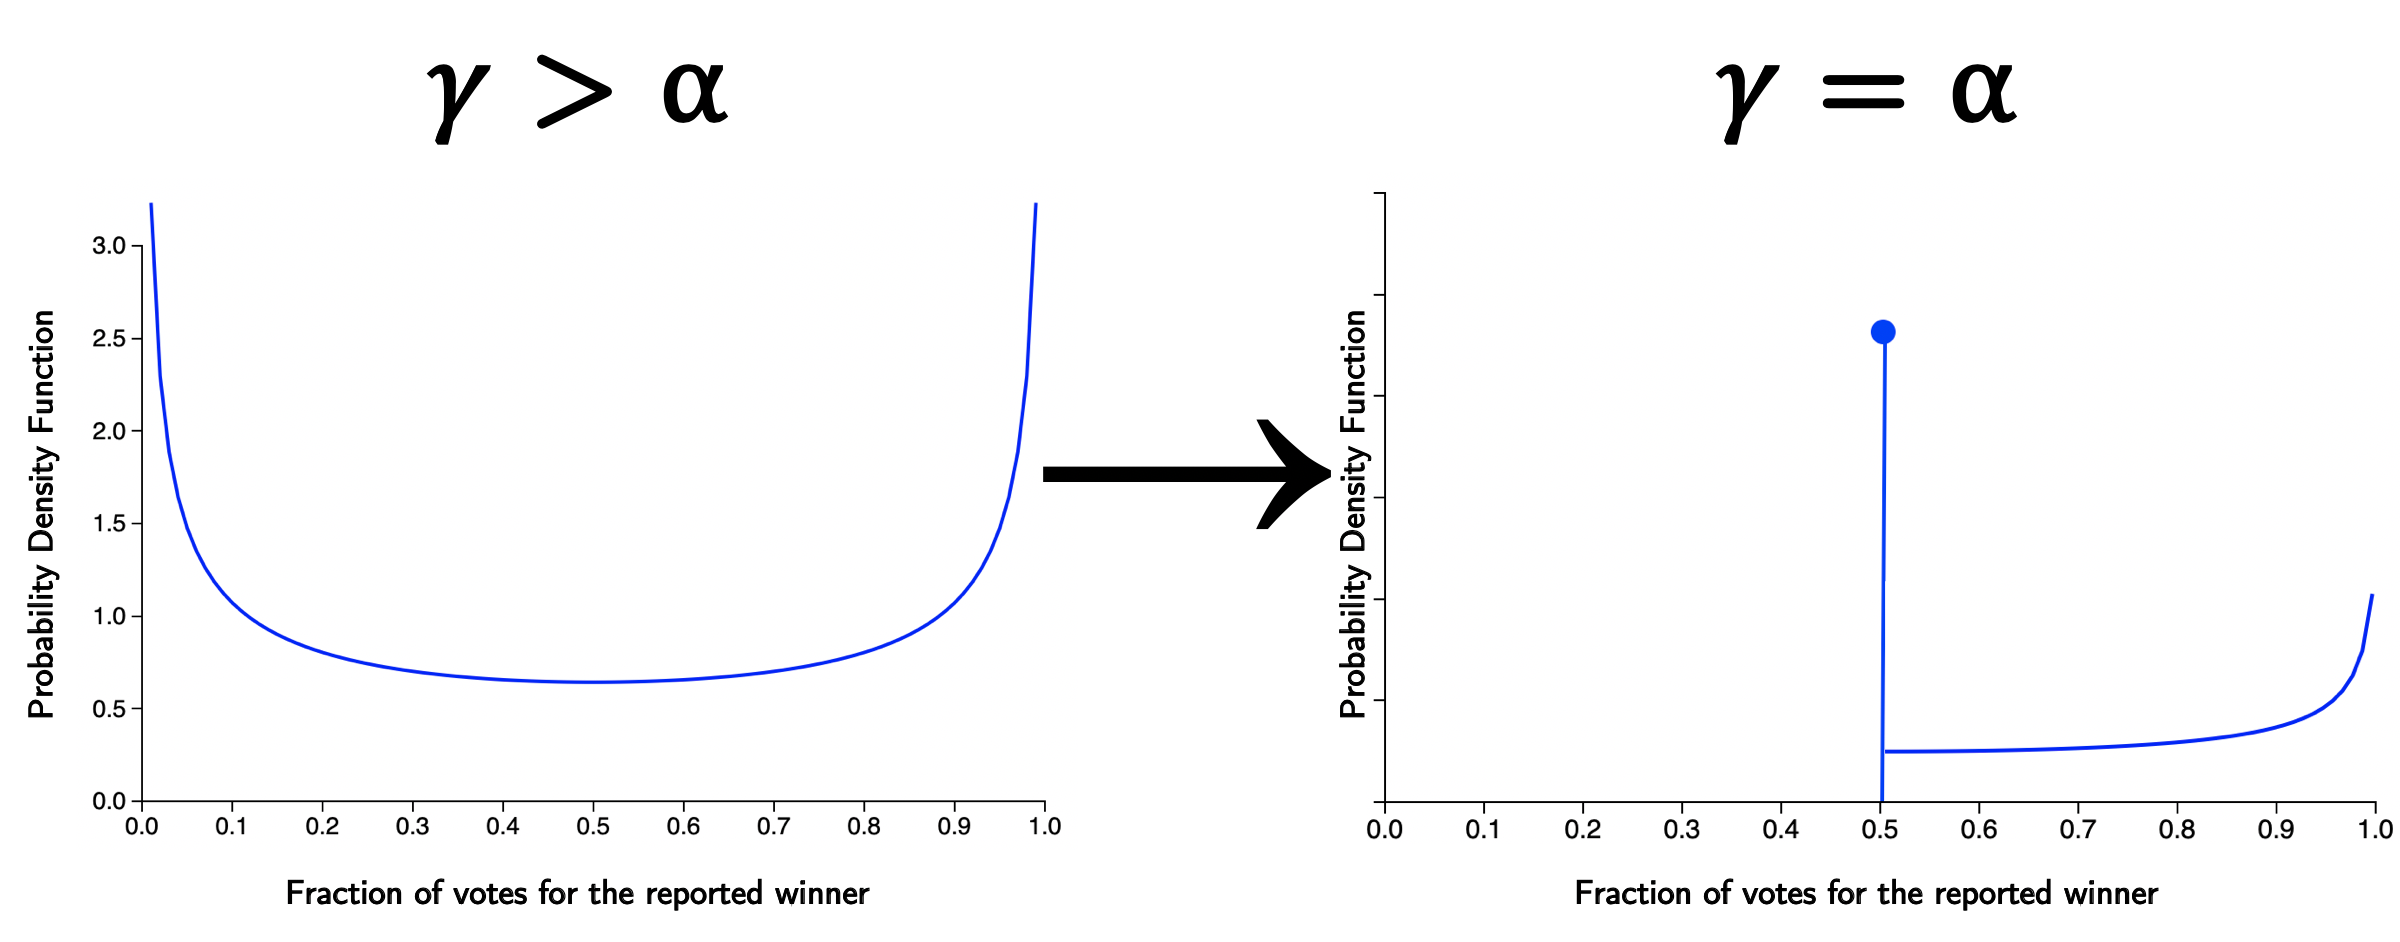
\includegraphics[width=300pt]{BRLA_Prior.png}
    \caption{On the left: $f_X$, the right: $f_X^*$. Other priors, such as the uniform prior, can also be made risk limiting in this way.}
    \label{fig:my_label}
\end{figure}
\end{frame}

\begin{frame}{Stopping Rule and Efficiency of Bayesian RLAs}
\begin{figure}
    \centering
    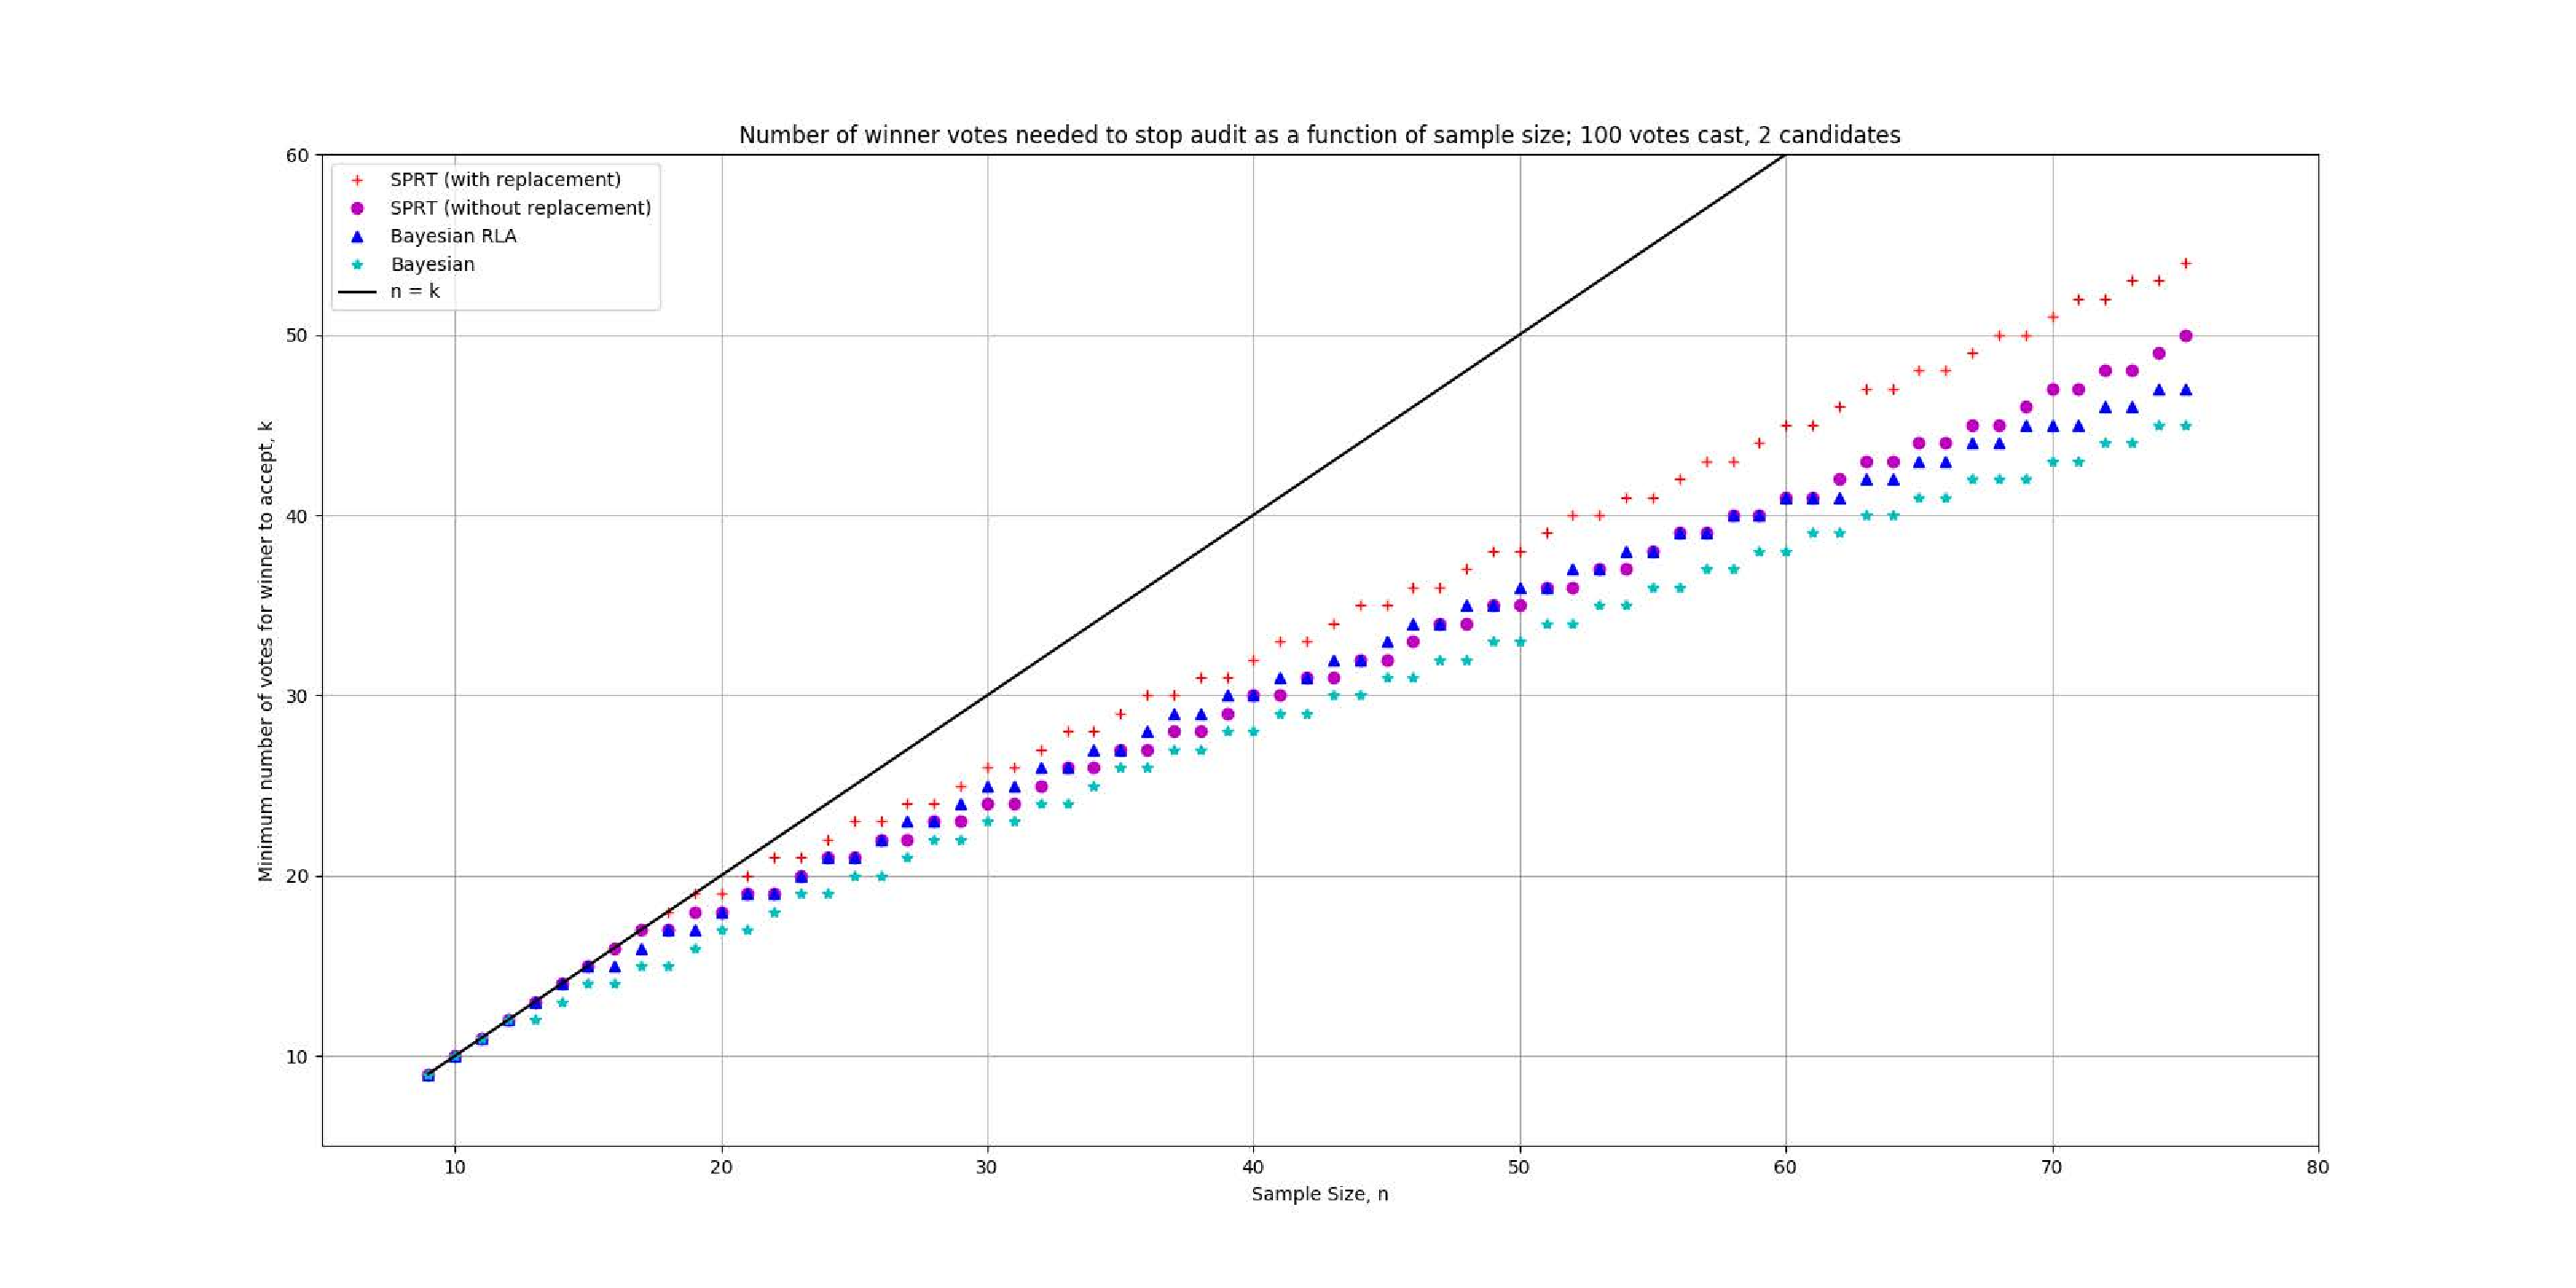
\includegraphics[width=320pt]{RLA_vs_Bayesian2.pdf}
    \caption{The stopping rules ($k_{min}(n)$) of the Bayesian RLA is compared to the Bayesian audit (uniform prior) and two flavors of the SPRT RLA, $p = .75$.}
    \label{fig:my_label}
\end{figure}
\end{frame}

\begin{frame}{Stopping Rule and Efficiency of Bayesian RLAs: Graph Observations}
\begin{itemize}
    \item The Bayesian audit required the fewest number of ballots to stop because it is not risk limiting.
    \vskip 1cm
    \item The Bayesian RLA required fewer ballots to stop than either flavor of the SPRT RLA, indicating a potential application of Bayesian RLAs in designing more efficient audits.
    \begin{itemize}
        \item These efficiency differences are in spite of the audits being (nominally) risk-limited at the same level!
    \end{itemize}
\end{itemize}
\end{frame}

\begin{frame}{Conclusions}
\begin{itemize}
    \item In general, Bayesian audits are not risk-limiting.
    \vskip 1cm
    \item But one can choose a prior so that a Bayesian polling audit (in the two-candidate case) is risk-limiting.
    \vskip 1cm
    \item The Bayesian RLA provides a theoretically unifying framework, and holds promise as a means of improving audit efficiency.
\end{itemize}
\end{frame}

\begin{frame}{Future Directions}
\begin{itemize}
    \item How can we treat invalid votes in a risk-limiting manner in the Bayesian RLA framework?
    \vskip 1cm
    \item How can we extend the Bayesian RLA to
    \begin{itemize}
        \item other types of audits, such as ballot and batch comparison audits?
        \item other types of elections, such as those with multiple candidates?
    \end{itemize}
\end{itemize}
\end{frame}

\end{document}